\documentclass[kpfonts]{patmorin}
\usepackage{pat}
\usepackage{paralist}

\usepackage[utf8]{inputenc}

\usepackage{graphicx}

\setlength{\parskip}{1ex}


\DeclareMathOperator{\sn}{sn}
\DeclareMathOperator{\qn}{qn}

\renewcommand{\SS}{\mathcal{S}}


\newcommand{\aref}[1]{(X\ref{a:#1})}
\newcommand{\alabel}[1]{\label{a:#1}}

\title{\MakeUppercase{Optimal Adjacency-Labelling Schemes for Planar Graphs}}
\author{Barbados Folks}

\begin{document}
\maketitle

\begin{abstract}
  We describe an adjacency labelling-scheme for $n$-vertex planar graphs that assings each vertex a label of length $\log n+o(\log n)$.
\end{abstract}

\section{Introduction}


For a graph $G$, we use $V(G)$ and $E(G)$ to denote the vertex and edge sets of $G$.  We use $|G|$ as a shorthand for $|V(G)|$.

A \emph{prefix-free code} $c:X\to\{0,1\}^*$ is a one-to-one function in which $c(x)$ is not a prefix of $c(y)$ for any two distinct $x,y\in X$.
The following is an old result of Elias:

\begin{lem}
    There exist a prefix-free code $\gamma:\N\to\{0,1\}^*$ such that, for each $i\in\N$, $|\gamma(i)|\le \log(i+1)+O(\log\log i)$.
\end{lem}

A \emph{binary tree} $T$ is a rooted binary tree in which each node is either the left or right child of its parent and any node has at most one left and at most one right child.  

Let $T$ be a binary tree and let $v_0,\ldots,v_{r}$ be a path from the root $v_0$ of $T$ to some node $v_r$ (possibly $r=0$).  Then the \emph{signature} of $v_r$ in $T$, denoted $\sigma_T(r)$ is a binary string $b_1,\ldots,b_r$ where $b_i=0$ if and only if $v_{i}$ is the left child of $v_{i-1}$.  (Note that the signature of the root $v_0$ of $T$ is the empty string,  $\sigma_T(v_0)=\varepsilon$.)

A \emph{binary search tree} $T$ is a binary tree  whose node set $V(T)\subset\R$ consists of numbers and that has the BST property:  For any node $x$ that is a left-child of its parent $p$, $x<p$ and for any node $y$ that is a right-child of its parent $p$, $p<y$.  

\begin{obs}\obslabel{lexicographic}
  If $T$ is a binary search tree then, for any $x,y\in V(T)$, $x<y$ if and only if $\sigma_T(x)$ is lexicographically less than $\sigma_T(y)$.
\end{obs}


The following is an easily and often-used result obtainable by a greedy strategy: 

\begin{lem}\lemlabel{biased-bst}
  For any $w:\{1,\ldots,n\}\to\R^+$, there exists a binary search tree $T$ containing $\{1,\ldots,n\}$ such that, for each $i\in\{1,\ldots,n\}$, $d_T(i)\le\log(W/w(i))$, where $W=\sum_{i=1}^n w(i)$.
\end{lem}

To construct the tree in \lemref{biased-bst}, choose the root of $T$ to be the unique node $x\in\{1,\ldots,n\}$ such that $\sum_{z=1}^{x-1} w(i)\le W/2$ and $\sum_{z=x+1}^{n} w(i)< W/2$.  Then recurse on $\{1,\ldots,x-1\}$ and $\{x+1,\ldots,n\}$ to obtain the left and right subtrees respectively.

The following fact about binary search trees is useful, for example, in the deletion algorithms for binary search trees:

\begin{lem}\lemlabel{predecessor-encoding}
  Let $T$ be a binary search tree and let $x,y\in V(T)$ be such that $x<y$ and there is no node $z\in V(T)$ such that $x<z<y$ (i.e., $x$ and $y$ are consecutive in the sorted order of $V(T)$).  Then
  \begin{enumerate}
    \item (if $x$ has no left child) $\sigma_T(y)$ is obtained from $\sigma_T(x)$ by removing all trailing 0's and the last 1; or
    \item (if $x$ has a left child) $\sigma_T(y)$ is obtained from $\sigma_T(x)$ by appending a 0 followed by $s:=d_T(y)-d_T(x)-1$ 1's.
  \end{enumerate}
\end{lem}

Putting the a few of the preceding results together we obtain the following use coding result:

\begin{lem}\lemlabel{row-code}
  The exists a function $A:(\{0,1\}^*)^2\to\{-1,1,\perp\}$ such that, for any $h\in\N$, and any $w:\{1,\ldots,h\}\to\R^+$ there is a prefix-free code $\alpha:\{1,\ldots,h\}\to \{0,1\}^*$ such that 
  \begin{compactenum}
    \item for each $i\in\{1,\ldots,h\}$, $|\alpha(i)|=\log W -\log w(i) + O(\log\log h)$; and
    \item for each distinct $i,j\in\{1,\ldots,h\}$, 
    \[   A(\alpha(i),\alpha(j)) 
    = \begin{cases}
       1 & \text{if $j=i+1$} \\
       -1 & \text{if $j=i-1$} \\
       \perp & \text{otherwise}
      \end{cases}
      \]
    \end{compactenum}
\end{lem}


\begin{proof}
  Define $w':\{1,\ldots,h\}\to \R^+$ as $w'(i)=w(i)+W/h$ and let $W':=\sum_{i=1}^h w'(i)=2W$.
  Using \lemref{biased-bst}, construct a biased binary search tree $T$ on $\{1,\ldots,h\}$ using $w'$ so that 
  \[   
    d_T(i)\le\log (2W)-\log(w(i)+W/h) \le \log W-\log w(i)+1 \enspace .
  \]
  Also
  \[
  d_T(i)\le\log (2W)-\log(w(i)+W/h) \le \log W-\log (W/h)+1 \le \log h + 1\enspace .
  \]
  for each $i\in\{1,\ldots,h\}$.  The code $\alpha(i$) for $i$ consists of three parts.  The first part, $\gamma(|\sigma_T(i)|)$, encodes the length of the path from the root to $i$ in $T$. The second part $\sigma_T(i)$ encodes the left/right turns along this path.  
  
  The third part $\delta(i)$ of $\alpha(i)$ is the encoding implicit in \lemref{predecessor-encoding}.  That is $\delta(i)$ consists of
  a single bit indicating whether $i$ has a left-child in $T$ and, in case $i$ does have a left-child, an Elias encoding of the value $s=d_T(i-i)-d_T(i)-1$.  More precisely $\delta(i)=0$ or $\delta(i)=1,\gamma(s)$.  The length of $\delta(i)$ is at most $1+O(\log(s+1))=O(\log\log h)$.

  The function $A$ is now given by a simple algorithm: Given $\alpha(i)$ and $\alpha(j)$ we extract and lexicographically compare $\sigma_T(i)$ and $\sigma_T(j)$.  Assume, for now that $\sigma_T(i)$ is lexicographically less than $\sigma_T(j)$ so that, by \obsref{lexicographic}, $i < j$.  Now using $\sigma_T(j)$ and $\delta(j)$, compute $\sigma_T(j-1)$.  If $\sigma_T(j-1)=\sigma_T(i)$ then output $1$, otherwise output $\perp$.
  In the case where $\sigma_T(i)$ is lexicographically greater than $\sigma_T(j)$ we proceed in the same manner, but reversing the roles of $i$ and $j$ and outputting $-1$ in the case where $\sigma_T(i-1)=\sigma_T(j)$.
\end{proof}

\section{Subgraphs of Grid Products}

We being with the special case where $G\subseteq H\boxtimes P$ is an $n$-vertex graph where $H$ is a path.  The best way to think of this is to let $P=1,\ldots,h$, $H=1,\ldots,m$ so that each vertex of $G$ is a pair $(x,y)\in[m]\times [h]$.  

For each $y\in\{1,\ldots,h\}$, we let $L_y=\{x:(x,y)\in V(G)\}$.  The idea behind our approach is to have a sequence $T_1,\ldots,T_h$ of balanced binary search trees where, for each $y\in\{1,\ldots,h\}$,
\begin{enumerate}[(PR1)]
  \item $T_y$ contains (a superset of) $L_y\cup \{x-1:x\in L_y\}$;
  \item The height $h(T_y)$ of $T_y$ is $\log |T_y| + o(\log n)$;
  \item $W:=\sum_{y=1}^h |T_y| = O(n)$;
  \item If $x\in V(T_y)\cap V(T_{y+1})$, then $\sigma_{T_{y+1}}(x)$ can be obtained from $\sigma_{T_{y}}(x)$ with an additional $o(\log n)$ bits that we denote by $\nu_y(x)$.  More precisely, there is a (universal) function $B:(\{0,1\}^*)^2\to\{0,1\}^*$ such that $B(\sigma_{T_{y}}(x), \nu_y(x))=\sigma_{T_{y+1}}(x)$
\end{enumerate}
If we can find such a sequence of binary search trees, then things become easy.  Given $G$ and $T_{1},\ldots,T_h$ we use \lemref{row-code} with the weight function $w(y):=|T_y|$ to construct a code $\alpha:\{1,\ldots,h\}\to\{0,1\}^*$ where
\[  
  |\alpha(y)| = \log W-\log|T_y| + O(\log\log h) = \log n - \log|T_y| + o(\log n)
\]
for each $y\in\{1,\ldots,h\}$.  Every vertex $v=(x,y)\in V(G)$ receives a label consisting of the following:
\begin{enumerate}
  \item $\alpha(y)$;
  \item $\gamma(|\sigma_{T_y}(x)|)$ and $\sigma_{T_y}(x)$;    
  \item $\delta_{T_y}(x)$;
  \item $\nu_y(x)$; and
  \item an array $a(v)$ of $8$ bits indicating whether each of the edges between $(x,y)$ and $(x\pm 1,y\pm 1)$ are present.  (Note that some of these 8 vertices may not even be present in $G$ in which case the resulting bit is set to 0 since the edge is not present in $G$.)
\end{enumerate}
The two major components of this label are $\alpha(y)$ and $\sigma_{T_y}(x)$ which, together have length $\log n + o(\log n)$.  The three remaining components each have size $o(\log n)$.

Given the labels of $w_1=(x_1,y_1)$ and $w_2=(x_2,y_2)$ we can test if they are adjacent as follows: Using \lemref{row-code} with $\alpha(y_1)$ and $\alpha(y_2)$, determine which of the following applies:
\begin{enumerate}
  \item $|y_1-y_2|\ge 2$: In this case we immediately conclude that $w_1$ and $w_2$ are not adjacent.  
  
  \item $y_1=y_2$: In this case, let $y:=y_1=y_2$ and $T:=T_y$ and lexicographically compare $x_1$ and $x_2$ to determine (without loss of generality) that $x_1<x_2$.  Using $\sigma_{T}(x_2)$ and $\delta_{T}(x_2)$, compute $\delta_{T}(x_2-1)$.  If $\delta_{T}(x_2-1)\neq \delta_T(x_1)$ then immediately conclude that $w_1$ and $w_2$ are not adjacent.  Otherwise, we know that $x_1=x_2-1$ and $y_1=y_2$ so use the relevant bit of $a(w_1)$ (or $a(w_2)$) to determine if $w_1$ and $w_2$ are adjacent in $G$.
  
  \item $y_1=y_2-1$: In this case, use $\sigma_{T_{y_1}}(x_1)$ and $\nu_{y_1}(x_1)$ to compute $\sigma_{T_{y_2}}(x_1)$.  Now let $y:=y_2$, $T:=T_{y}$, and proceed as in the previous case (but consulting a different bit of $a(w_1)$ in the last step.)
  
  \item $y_1=y_2+1$: In this case, use $\sigma_{T_{y_2}}(x_2)$ and $\nu_{y_2}(x_2)$ to compute $\sigma_{T_{y_1}}(x_2)$.  Now let $y:=y_1$, $T:=T_{y}$, and proceed as in the previous case (but consulting a different bit of $a(w_1)$ in the last step.)
\end{enumerate}

Thus, all that remains is to find a sequence of binary search trees $T_1,\ldots,T_h$ with properties (PR1)--(PR4). This is a data structuring problem and we can use techniques from data structures to solve it.

\subsection{Fractional Cascading}

For disjoint sets $X,Y\subset \R$ we say that $X$ \emph{$k$-chunks} $Y$ if, for any $k$-element subset $S\subseteq Y$, there exists $x\in X$, such that $\min(S)< x<\max(S)$. 

For each $y\in\{1,\ldots,h\}$, let $L^-_y:=L_y\cup \{x-1:x\in L_y\}$ and observe that $|L^-_y|\le 2|L_y|$, so $\sum_{y=1}^h|L^-_y| \le 2n$.  The following lemma is a form of fractional cascading:

\begin{lem}\lemlabel{fractional}
  There exists universal constants $a,b\ge 1$ and $V_1,\ldots,V_h$ such that, 
  \begin{compactenum}
    \item for each $y\in\{1,\ldots,h\}$, $V_y\supseteq L^-_y$;
    \item for each $y\in\{1,\ldots,h-1\}$, $V_y\cup V_{y+1}$ $a$-chunks $V_{y+1}\setminus V_y$ and $V_y\setminus V_{y+1}$; and
    \item $\sum_{y=1}^h |V_y|\le bn$.
  \end{compactenum}
\end{lem}

Condition~2 in \lemref{fraction} has the following interpretation:  If we sort $V_y\cup V_{y+1}$, then we never see $a$ consecutive elements that only belong only to $V_y$ nor do we ever see $a$ consecutive elements that belong only to $V_{y+1}$.

We will use \lemref{fractional} to creating the sequence of binary search trees $T_1,\ldots,T_h$ where $V(T_y)=V_y$ for each $i\in\{1,\ldots,h\}$.  Condition~2 in \lemref{fractional} is what will ultimately make it possible to have $T_y$ and $T_{y+1}$ sufficiently similar so that, for any $x\in V_y\cap V_{y+1}$, there will be an $o(\log n)$-bit description of how to modify $\sigma_{T_y}(x)$ in order to obtain $\sigma_{T_{y+1}}(x)$.

\subsection{Bulk Deletions}

\begin{lem}\lemlabel{deletion-prefix}
  For any binary search tree $T$ and any $X\subseteq V(T)$, there exists a binary search tree $T'$ with $V(T')=V(T)\setminus X$ such that, for every $x\in V(T')$, $\sigma_{T'}(x)$ is a prefix of $\sigma_{T}(x)$.
\end{lem}

\begin{proof}
  It suffices to prove this for a singleton set $X$ containing one element $z$ since, for larger $X$ we can remove the values from $T$ one at a time.  
  
  The proof is by induction on $|T|$. If $|T|=1$, then the claim is vacuous since $V(T')=\emptyset$.  Therefore assume $|T|\ge 2$.  If $z$ is leaf in $T$, then use $T'=T-\{z\}$ and the result is trivial: $\sigma_{T'}(x)=\sigma_T(x)$ for every $x\in V(T')$.  
  
  Otherwise, $z$ has at least one child.  Without loss of generality, assume $z$ has a non-empty left subtree $T_l$.  Then the largest node $y$ in $V(T_l)$ is the largest value in $V(T)$ that is less than $z$. Inductively remove $y$ from $T_l$ to obtain $T_l'$ and make this the left child of $z$.  Now replace $z$ with $y$ to obtain $T'$.  
  
  That $T'$ is indeed a binary search tree is straightforward to verify.  All that remains is to prove that $\sigma_{T'}(x)$ is a prefix of $\sigma_T(x)$ for every $x\in V(T')$. There are three cases:
  \begin{enumerate}
    \item $x=y$: Since $z$ is an ancestor of $y$ in $T$, $\sigma_{T'}(y)=\sigma_T(z)$ is a prefix of $\sigma_T(y)$.  
    
    \item $x\in V(T)\setminus\{z\}\setminus V(T_l)$: In this case $\sigma_T(x)=\sigma_{T'}(x)$.  
    
    \item $x\in V(T_l')$: In this case, $\sigma_{T'}(x)=\sigma_{T}(z),0,\sigma_{T_l'}(x)$ and $\sigma_T(x)=\sigma_{T}(z),0,\sigma_{T_l}(x)$.  By induction, $\sigma_{T_l'}(x)$ is a prefix of $\sigma_{T_l}(x)$, so $\sigma_{T'}(x)$ is a prefix of $\sigma_T(x)$. \qedhere
  \end{enumerate}
\end{proof}

\lemref{deletion-prefix} is useful because it means that, for any particular node of $x$ of $T_y$, the net effect of all the deletions performed when moving from $T_y$ to $T_{y+1}$ on $\sigma(x)$ can be encoded by a single integer in the range $\{0,\ldots,|\sigma_T(x)|\}$.  Using the $\gamma$-code, this requires only $O(\log |\sigma_T(x)|)$ bits.  If $T$ is at-all balanced, this is only $O(\log\log n)$ bits.

\subsection{Bulk Insertions}


\begin{lem}\lemlabel{chunked-addition}
  For any binary search tree $T$ and any set $Y\subset\R $ such that $V(T)$ $a$-chunks $Y$, there exists a binary search tree $T'$ with $V(T')=V(T)\cup Y$ that is a supergraph of $T$ and such that $h(T')=h(T)+O(\log a)$.
\end{lem}

\begin{proof}
  Search for each element $y\in Y$ in $T$ until the search path falls out of $T$.  This would be the natural place to add $y$ as a leaf to $T$.  This partitions $Y$ into $r:=|T|+1$ sets $Y_1,\ldots,Y_r$ and, since $V(T)$ $k$-chunks $Y$, each $Y_i$ has size at most $k$.  For each $Y_i$ construct a binary search tree $T_i$ of height at most $\log a$ and attach this to the appropriate location in $T$ to obtain $T'$.
\end{proof}

\lemref{chunked-addition} is useful because the set of values $Y$ that are present in $T_{y+1}$ but not in $T_y$ are $a$-chunked by $V(T_y)$. Therefore, we can perform all the additions required to move from $T_y$ to $T_{y+1}$ in such a way that $\sigma_{T_y}(x)=\sigma_{T_{y+1}}(x)$ for every $x\in L(y)\cap L(y+1)$.  

\subsection{Tree Splitting}

\begin{lem}\lemlabel{split}
  Let $T$ be a binary search tree and let $x$ be any node of $T$.  Then there exists a binary search tree $T'$ with $V(T')=V(T)$ whose root is $x$ and such that, for each node $y\in V(T')$, $\sigma_{T'}(y)$ is obtained by replacing a prefix of $\sigma_{T}(y)$ with a binary string from the set $\{\varepsilon\}\cup \{01^r:r\in\{0,\ldots,h(T)\}\cup \{10^r:r\in\{0,\ldots,h(T)\}$.  Furthermore $h(T')\le h(T)+1$.
\end{lem}

\begin{proof}
Proof by (crappy) illustration:
  \begin{center}
    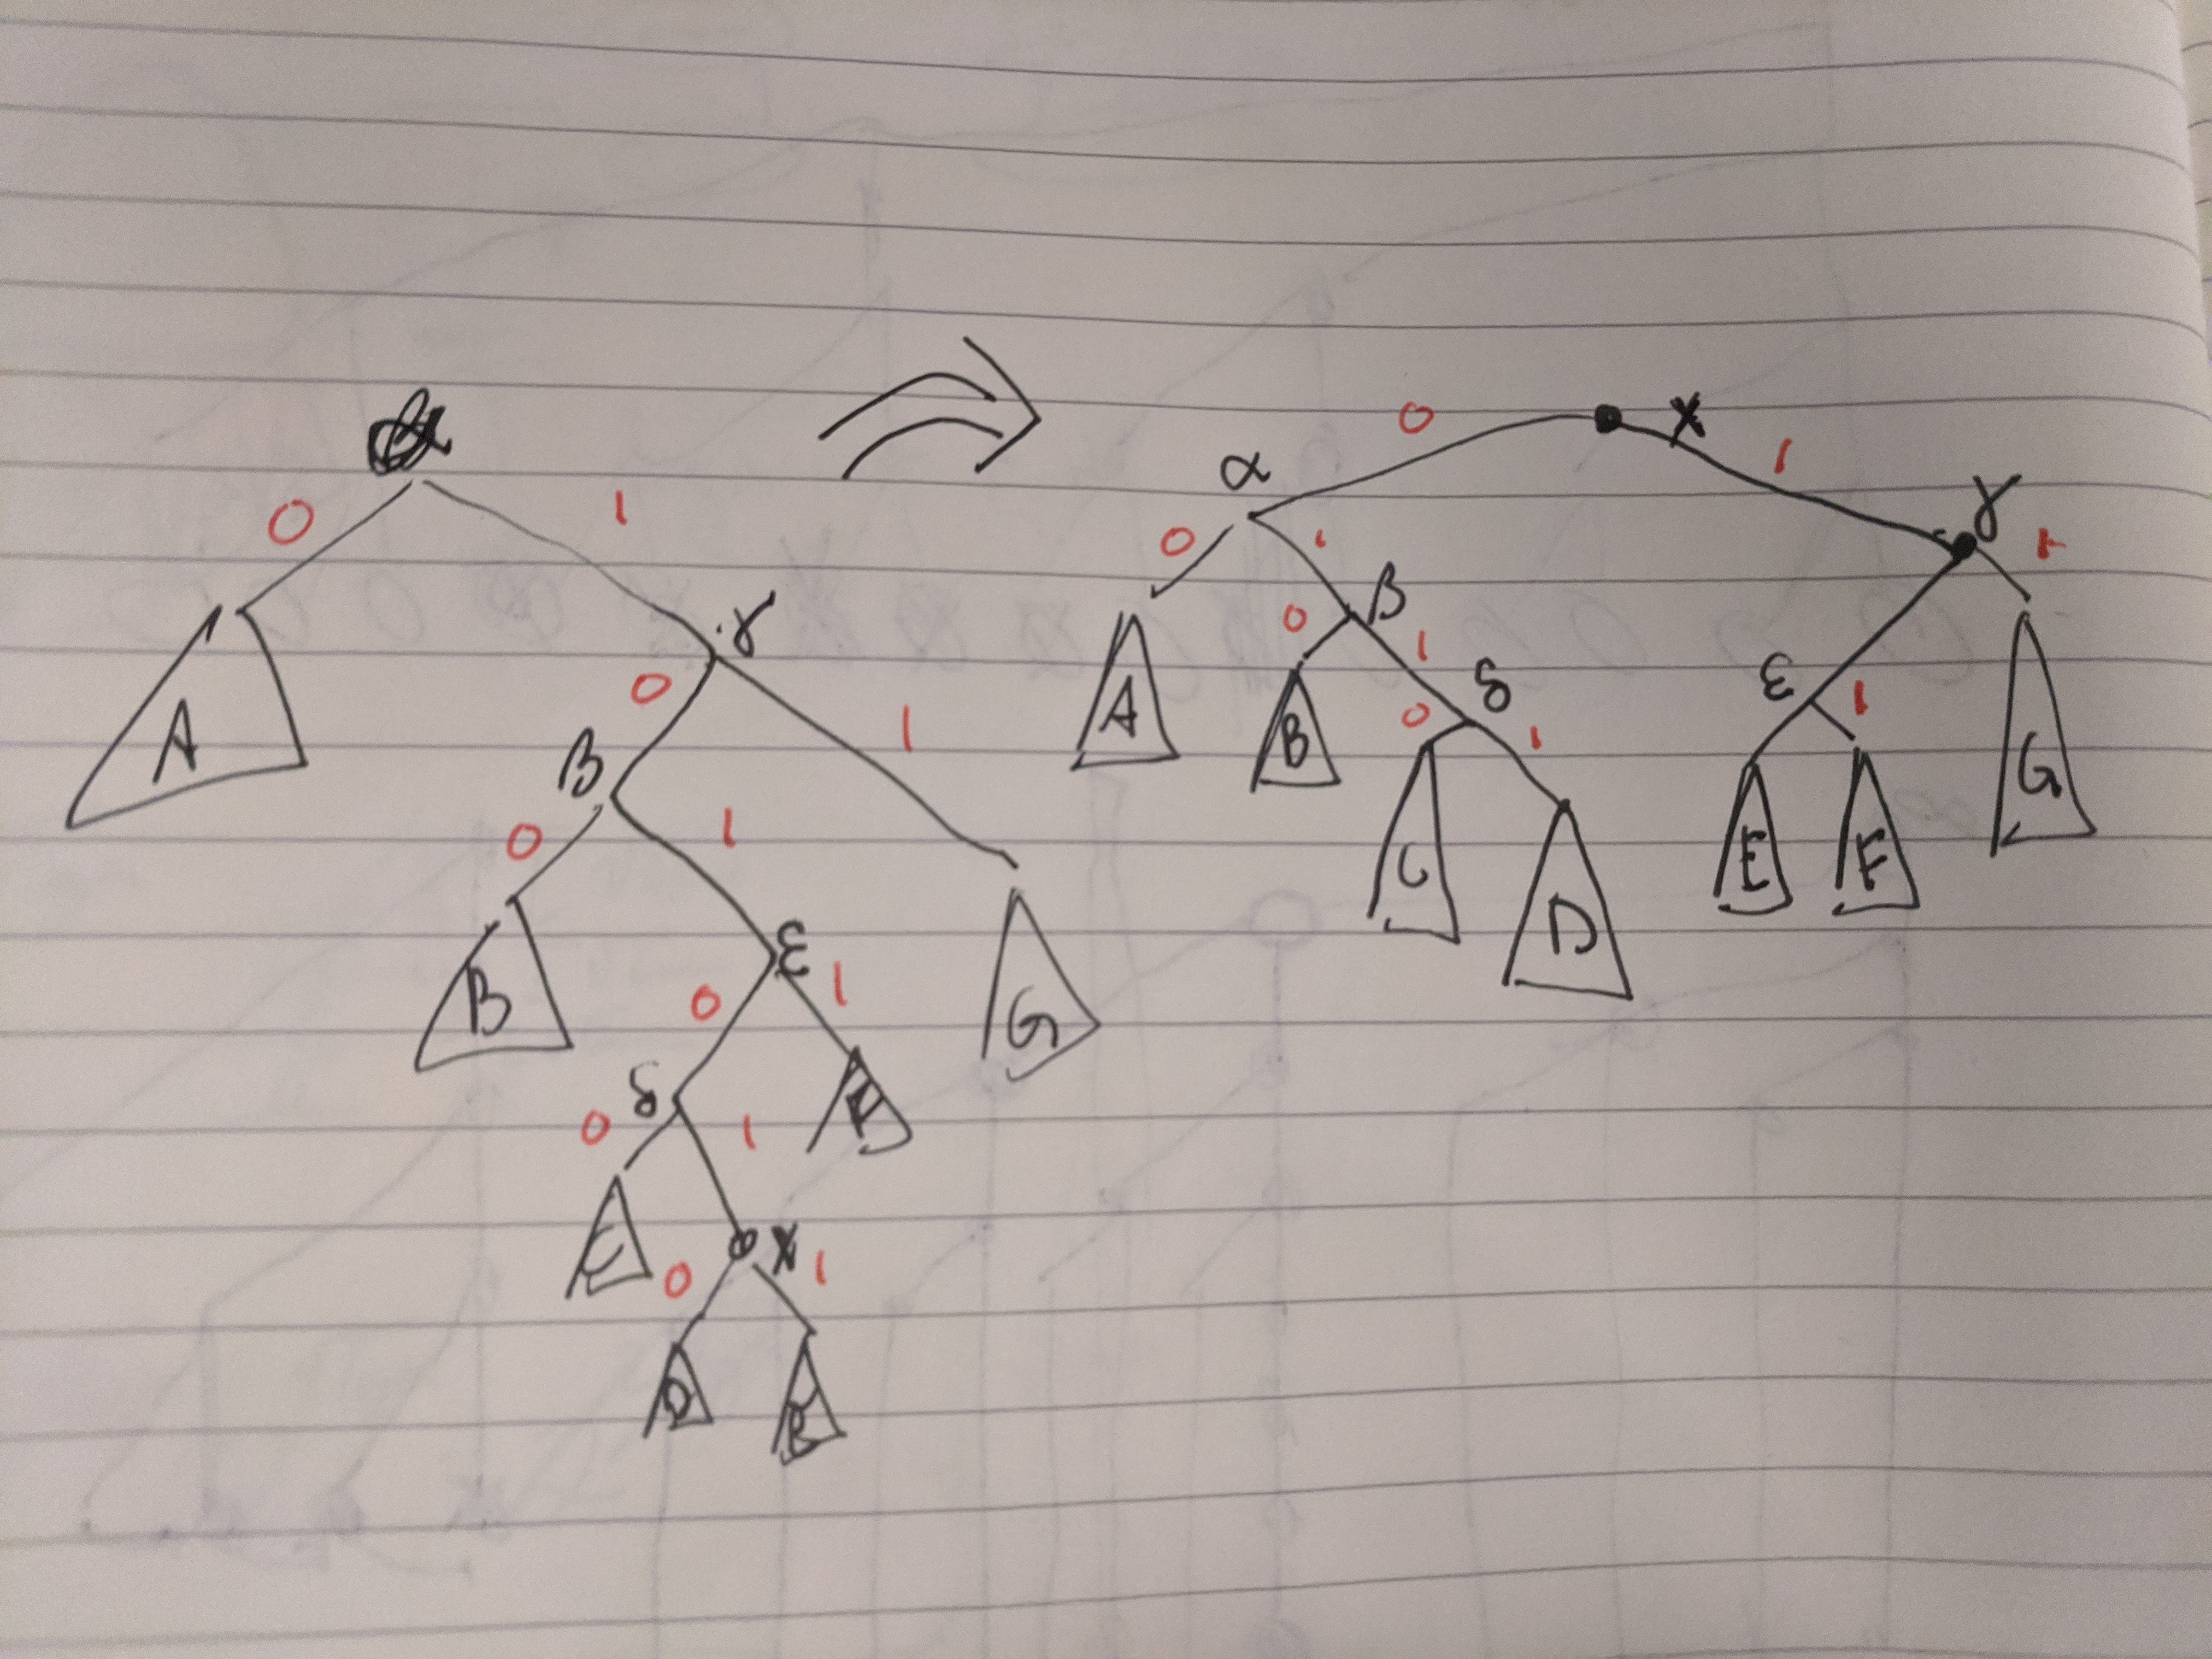
\includegraphics[width=.6\textwidth]{images/split}
  \end{center}
\end{proof}

\lemref{split} allows us to perform a perfect split at the root of $T$ and still maintain an $O(\log h(T))$-length description of the changes required to obtain $\sigma_{T'}(x)$ from $\sigma_T(x)$.  \lemref{split} can be applied recursively to obtain the following result:

\begin{lem}\lemlabel{multi-split}
  Let $c>1$, $k\ge 1$, and let $T$ be a binary search tree.
  % . such that, for each subtree $T_i$, $i\in\{1,\ldots,m\}$ of $T$ rooted at a depth-$k$ node, $|T_i|\le |T|/(c2^k)$.  

  Then there is a binary search tree $T'$ with $V(T')=V(T)$ in which
  \begin{compactenum}
    \item  each of the subtrees $T_i'$, $i\in\{1,\ldots,m'\}$ rooted at a depth-$k+1$ node has size at most $|T|/2^k$;
    
    \item $h(T')\le h(T)+\log c+1$; and
    
    \item for each $x\in V(T)$, there exists an $O(k+\log a\log h(T))$-bit description of the changes required to create $\sigma_{T'}(x)$ from $\sigma_T(x)$.
  \end{compactenum}
\end{lem}

\begin{proof}
  Let $Y\subset V(T)$ be the set of at most $2^k-1$ nodes of $T$ of depth less than $k$.  Then $T-Y$ is a forest consisting of $m\le 2^{k}$ trees $T_1,\ldots,T_m$.  Each such tree $T_i$ has height at most $h(T)-k$.
  
  Select the nodes $X:=\{x_1,\ldots,x_{2^k}-1\}$ of $T$ where each $x_j$ has rank $\lfloor j|T|/2^k\rfloor$.  For each $i\in\{1,\ldots,2^k-1\}$ and each $x\in X\cap V(T_i)$, apply \lemref{split} to the subtree $T_i$ with the value $x$ to obtain a new subtree $T_{i}'$.  In $T_i'$, the nodes in $X\cap V(T_i)$ induce a connected subtree that contains the root. Now, $T_i'-(X\cap V(T_i))$ is a forest consisting of trees trees $T'_{i,1},\ldots,T'_{i,d_i}$ each of which has height at most $h(T_i) \le h(T)-k$.  

  Doing this for each $T_i$ creates a forest of $\ell\le 2^{k+1}$ trees $T^@_1,\ldots,T^@_{\ell}$ each having height at most $h(T_i)\le h(T)-k$.  Now, form a complete binary search tree $T_0'$ from the nodes in $X\cup Y$.  $T_0'$ contain at most $2(2^k-1)<2^{k+1}-1$ nodes, so $h(T'_0)\le k$.  Next attach each of $T^@_1,\ldots,T^@_\ell$ to the appropriate location in $T'_0$ to obtain the tree $T'$ we want.  Observe that $T'$ has height at most $h(T'_0)+1+\max_i h(T^@_i)\le k+1+h(T)-k=h(T)+1$.
  
  For the final condition, observe that, for each each node $x\in X\cup Y$ we can explicitly write $\sigma_{T'}(x)$ using $\log k+1 + O(\log\log k)$ bits.  For each $x\in V(T)\setminus(X\cup Y)$, $x$ is included in at most $\log c$ subtrees on which \lemref{split} was applied so the necessary changes to $\sigma_T(x)$ can be encoded using $O(\log c\log h(T))$ bits and the path from the root of $T'$ to the root of the subtree $T^@_i$ containing $x$ can be encoding using $k+1+O(\log k)$ bits.
\end{proof}

\subsection{Rebalancing}

We can now describe the sequence of binary search trees $T_1,\ldots,T_h$ required by the encoding scheme. The tree $T_1$ is a perfectly balanced binary search tree on node set $V_1$.  To obtain $T_2$, we first use \lemref{chunked-addition} to insert the elements of $V_2\setminus V_1$ into $T_1$ to obtain a binary search tree tree $T_1'$ with node set $V_1\cup V_2$.   Note that, since $V_1\cap V_2$ $a$-chunks $V_2$, these insertions do not add more than $(a-1)\cdot(|T_1|+1)\le 2(a-1)|T_1|$ nodes. Therefore $|T_1'|\le 2a|T_1|$.  Also $h(T_1')\le h(T_1)+\log a$.  

If $|T_1'|<2^k$ (for some $k\in o(\log n)$ to be specified later), then life is easy.  We make $T_2$ a perfectly balanced binary search tree and, for each node $x$ we store $\sigma_{T_1}(x)$ and $\sigma_{T_2}(x)$ explicitly.  In this case $\nu_1(x)$ consists of a few code bits, $\gamma(|\sigma_{T_1}(x)|)$, $\sigma_{T_1}(x)$, $\gamma(|\sigma_{T_2}(x)|)$, and $\sigma_{T_2}(x)$.  In this case we then proceed the same way beginning from $T_2$.

On the other hand, if $|T_1'|\ge 2^k$ , then we apply \lemref{multi-split} to $T_1'$ to obtain a new tree $T_1''$ of height at most $h(T_1')+O(\log a)$.  Consider the $2^{k+1}$ subtrees of $T_1''$ rooted at the depth-$k+1$ nodes of $T_1''$.  Each of these subtrees has size at most $|T_1''|/2^k\le 2a|T_1|/2^k$.  Next we apply use \lemref{deletion-prefix} to delete elements of $V_1\setminus V_2$ and we define $T_2$ to be the resulting tree.  Deletions do not increase the depth of any node, so $h(T_2)\le h(T_1'')\le h(T_1')+1\le h(T_1)+1+\log a$.  For each node $x\in T$, we make $\nu_1(x)$ by using the code described in \lemref{multi-split} followed by the code described in \lemref{deletion-prefix}.

Next, to obtain $T_3$ from $T_2$ we first use \lemref{chunked-addition} to insert the elements of $V_3\setminus V_2$ into $T_2$ to obtain a binary search tree $T_2'$ with node set $V_2\cup V_3$.   Again, these insertions do not add more than $2a|T_2|$ nodes and $h(T_2')\le h(T_2)+\log a\le h(T_1)+1+2\log a$.  Now, $T_2'$ has at most $2^{k+1}$ subtrees whose roots have depth $k+1$ and each of these subtrees has size at most $(2a)^2|T_1|/2^k$.  If $(2a)^2|T_1|/2^k < 2^k$ then we rebuild each of these subtrees into a perfectly balanced binary search tree of height at most $k-1$.  Everything is easy and we can get away with $\nu_2(x)$ of size $O(k)$ and codes of length $O(k)\in o(\log n)$.  At this point we proceed from the beginning again, as if $T_3$ were $T_1$.

If $(2a)^2|T_1|/2^k > 2^k$, then we apply \lemref{multi-split} to each of the at most $2^{k+1}$ depth-$k+1$ subtrees of $T_2'$ to obtain a new tree $T_2''$.  The tree $T_2''$ has at most $2^{2(k+1)}$ subtrees rooted at depth-$2(k+1)$ nodes that each have size at most $a^2|V_1|/2^{2k}$. Now, $h(T_2'')\le h(T_2)+O(\log a)$. Again, we apply \lemref{deletion-prefix} to delete elements of $V_2\setminus V_3$ and we define $T_3$ to be the resulting tree.  The signatures of nodes in $T_3$ have length $h(T_1)+O(k+\log a)$.  Furthermore, for each node $x\in V(T_2'')$ there is only one application of \lemref{multi-split} on a subtree of $T_2'$ that contains $x$, so $\nu_2(x)$ has length $O(k+\log a\log h(T_2'))$.

After $r$ iterations of this kind, the subtrees rooted at nodes of depth $r(k+1)$ have size at most
\[
     f(r) := 2a\left(\frac{2a}{2^k}\right)^r|V_1|
\]
and have height at most $h(T_1)-r(k+1)+r(1+\log a)$.  Therefore $h(T_r)\le h(T_1)+r(1+\log a)$.

We quit if $f(r)<2^k$, which occurs when
\[
   r > \frac{k + \log |T_1| + \log(2a)}{(k-\log 2a)} \enspace .
\]
Observe that 
\[
   h(T_r) \le h(T_1)+r(1+\log a) \le h(T_1) + O(h(T_1)/k) = (1+O(1/k))\log|T_1|
\]
On the other hand, $|T_r|\ge |T_1|/a^r$, so
\[  \log |T_r| \ge \log|T_1| - r\log a \ge (1-O(1/k))\log|T_1| \]
Putting these things together, we see that 
\[
   h(T_r) \le (1+O(1/k))\log |T_r| \enspace .
\]
Therefore, for all $r$, $|\sigma_{T_r}(x)|\le (1+O(1/k))\log|T_r|$.  The size of $\nu_r(x)$ is $O(k+\log(h(T_r))$.  If we take $k=\sqrt{\log n}$, for example, then $h(T_r)=\log |T_r|+O(\sqrt{\log n})$ and $|\nu_r(x)|=O(\sqrt{\log n})$.  Thus we get a sequence of trees $T_1,\ldots,T_h$ that satisfy (PR2) with $h(T_y)=\log_|T_y| + O(\sqrt{\log n})$ and (PR4) with $|\nu_y(x)|=O(\sqrt{\log n})$.

In this way, we obtain an adjacency labelling scheme for any $n$-vertex graph $G\subseteq P\times P$.





% 
% 
% Unfortunately, the previous two results are not quite enough.  We must also ensure that height, $h(T_{y+1})$, of $T_{y+1}$ is $\log |T_{y+1}| + \tau$ where $\tau\in o(\log n)$.  Working in our favour is that the set $X$ of nodes that we delete when moving from $T_y$ to $T_{y+1}$ has size at most $|T_y|/2$, so $|T_{y+1}|\ge |T_y|/2$. Thus, without doing anything, we are already guaranteed that 
% \[  
%   h(T_{y+1})\le h(T_y)\le \log|T_y|+\tau \le \log|T_{y+1}| + 1 + \tau \enspace ,
% \]
% after deletion of the nodes in $V(T_y)\setminus V(T_{y+1})$. As discussed above, the addition of nodes $V(T_{y+1})\setminus V(T_y)$ increases the height of $T_y$ by at most $O(\log\log n)$, so after the deletions and additions, 
% \[  
%   h(T_{y+1})\le \log|T_{y+1}| + 1 + O(\log\log n) + \tau \enspace ,
% \]
% 
% Similarly, the set of nodes we add when moving from $T_y$ to $T_{y+1}$ is also bounded by the size of $T_y$.  So
% \[ |T_y|/2\le |T_{y+1}| \le 2|T_y| \]
% and there's more, but I'm out of time.

% At this point I'm running out of steam and time, but there seems to be many ways to make this work.  The point is that the transition from $T_y$ into $T_{y+1}$ involves two steps:
% \begin{enumerate}
%   \item deletion of at most half the values in $T_y$, no two of which are adjacent.
%   \item insertion of at most $|V(T_y)|$ elements, each pair of which is already separated by some element already in $T_y$.
% \end{enumerate}
% Before I chug through this, I need to look up some of the literature (or consult a specialist) about the simplest way to do this.

\section{So What?}

The obvious question is: Why do we care about labelling schemes for $n$-vertex subgraphs of $P\boxtimes P$? The answer is that we probably don't.  However, this idea could potentially extend to $n$-vertex subgraphs of $H\boxtimes P$ where $H$ has constant treewidth.  Indeed, it's not hard to imagine a data structure for a fixed $H$, that maintains a vertex-induced subgraph of $H$ and supports bulk insertions and deletions (subject to restrictions like those above) and has properties analagous to (PR1)--(PR4).

Also, even if this doesn't extend to the case where $G$ is an $n$-vertex subgraph of $H\boxtimes P$ for some $H$ of constant treewidth, David Wood makes the point that $n$-vertex subgraphs of $P\boxtimes P\boxtimes\cdots\boxtimes P$ are also interesting, because of \url{https://link.springer.com/article/10.1007/s00493-007-2183-y}.









% The decomposition of $G$ into vertical paths corresponds to the property that, for any $i\in\{1,\ldots,h\}$,
% $X_i:=\{j: (i,j)\in V(G)\}$ is a contiguous set of intervals.
% 
% 
% 
%  and imagine that $V(G)$ has a layering $L_1,\ldots,L_h$.
% 
% 
% In particular 




\end{document}



\hrule
We think of $k$-trees being constructed by the process of repeatedly attaching a vertex $v$ to a $k$-clique $a_1,\ldots,a_k$.  We call $a_1,\ldots,a_k$ the parents of $v$ and we order them in the order in which they appeared in the construction.  We call $a_i$ the $i$th parent of $v$.

\begin{lem}\lemlabel{k-tree-weighted}
  Let $H$ be a $k$-tree, let $w:V(H)\to\R^+$ be an assignment of non-negative weights to the vertices of $H$ and let $W=\sum_{v\in V(H)}w(v)$.  Then $H$ has an adjacency-labelling scheme $\varphi:V(H)\to \{0,1\}^*$ in which the label $\varphi(v)$ of $v$ has length $\log(W/w(v)) + O(k+k\log\log(W/w(v)))$ for every $v\in V(H)$.
  
  Furthermore for any vertex $v$ with parents $a_1,\ldots,a_k$ the labels $\varphi(v)$ and $\varphi(a_i)$ are sufficient to determine that $\varphi(a_i)$ is the $i$th parent of the node whose label is $v$.
\end{lem}

\begin{proof}
  This is just a version of the labelling scheme for $k$-trees that uses weighted separating sets. TODO: Check if this can be simplified using tools from coding-theory so that we don't need to group nodes into separator sets of size $\log n$.  In particular, I think $(2/3)$-separators are good enough if combined with the right codes.
\end{proof}

\begin{lem}\lemlabel{partial-ktree-weighted}
  Let $H$ be a partial $k$-tree, let $w:V(H)\to\R^+$ be an assignment of non-negative weights to the vertices of $H$ and let $W=\sum_{v\in V(H)}w(v)$.  Then there exists an adjacency labelling scheme for $H$ in which the label of $v$ has length $\log(W/w(v)) + k\cdot(1+ o(\log(W/w(v))))$ for every $v\in V(H)$.
\end{lem}

\begin{proof}
  Apply \lemref{k-tree-weighted} to an encompassing $k$-tree of $H$ and give each vertex $v$ an additional $k$ bit array $b_1,\ldots,b_k$ where $b_i$ indicates if the edge between $v$ and its $i$th parent is actually in $H$ or not.
\end{proof}

\begin{lem}
  Let $G$ be an $n$-vertex planar triangulation.  Then $G$ has an adjacency-labelling scheme $\varphi(V)\to\{0,1\}^{\log n + o(\log n)}$.
\end{lem}

\begin{proof}
  Let $T$ be a BFS tree of $G$, let $\mathcal{P}=\{P_1,\ldots,P_r\}$ be a partition of $V(G)$ into vertical paths in $T$ such that $H:=G/\mathcal{P}$ is a partial 8-tree.  Let $H^+$ be some encompassing 8-tree of $H$ and let $x_1,\ldots,x_r$ be the vertices of $H^+$ ordered by the order in which they appear when constructing $H^+$.
  
  For each $i\in\{1,\ldots,r\}$ set $r(x_i)=\max\{2,\lceil\log_2 |P_i|\rceil\}$, and $w(x_i):=2^{r(x_i)}$.  Note that $w(x_i)\le 4|P_i|$ for each $i\in\{1,\ldots,r\}$, so $W:=\sum_{v\in V(H)} w(v)\le 4n$.
  
  The label of each node $u\in V(G)$ will have several parts.  For each $i\in\{1,\ldots,r\}$ and each $u\in P_i$, we store $r(u)$, which consists of $O(\log\log n)$ bits since $r(u)\in\{2,\ldots,\log n+1\}$.  Next, we store $\alpha(u)$, the label of the node $x_i$ in the adjacency-labelling of $H$ given by \lemref{partial-k-tree-weighted} using the weighting scheme $w:V(H)\to\R^+$ defined above.  The length of $\alpha(u)$ is at most
  \[  \log (W/w(x_i)) \le \log n - r(x_i) + crap \enspace . \]
  The second part of the label of $u$ is (the binary encoding of) $\delta(u):=d_T(u)\bmod 4w(x_i)$. This part consists of exactly $r(x_i)$ bits.
  
  Finally, the label of $u$ has $8$ more parts $\nu_1(u),\ldots,\nu_8(u)$ each consisting of 3 bits.  In the $k$-tree $H^+$, $x_i$ is adjacent to $8$ nodes\footnote{Skipping another detail here that this isn't true for $x_1,\ldots,x_8$} $x_{i_1},\ldots,x_{i_8}$ where $i_1<\cdots<i_8$.  For each $\ell\in\{1,\ldots,8\}$, there are three potential edges between $u$ and the vertices of $P_{i_\ell}$ at depths $d_T(u)-1$, $d_T(u)$ and $d_T(u)+1$.  The three bits in $\nu_{\ell}(u)$ indicate which of these three edges are actually present in $G$.
  
  Now, given the labels of two nodes $v$ and $w$, we check if $vw\in E(G)$ as follows.
  \begin{enumerate}
    \item Use $\alpha(v)$ and $\alpha(w)$ to check if the edge $x_ix_j\in E(H)$ where $v\in P_i$ and $w\in P_j$.  If not, then $G$ contains no edge between $P_i$ and $P_j$ and therefore $vw\not\in E(G)$ and we stop.  Otherwise we continue.
    \item Assume without loss of generality that $i < j$, so that $x_i$ is a parent of $x_j$ in the $k$-tree $H^+$.  From $\alpha(u)$ and $\alpha(v)$ we can detemine that $i<j$ and that $x_i$ is the $\ell$th parent of $x_j$ for some $j\in\{1,\ldots,8\}$.  Now, since $x_ix_j\in T$, we know that $|d_T(v)-d_T(w)|\le |P_i|+|P_j|-1$.  There are three cases to consider:
    \begin{enumerate}
      \item $r(x_i)=r(x_j)$.  In this case $|d_T(v)-d_T(w)|\le w(x_i)+w(x_j)-1 \le 2w(x_i)$.  In this case $d_T(v)-d_T(w)=a$ iff and only if $\delta(v)-\delta(v)\equiv a \pmod 4w(x_i)$.  In particular, this is true for $a\in\{-1,0,1\}$.  Therefore we can distinguish using $\delta(v)$ and $\delta(w)$, the four cases $d_T(v)-d_T(w)=-1$, $d_T(v)-d_T(w)=0$, $d_T(v)-d_T(w)=1$, or $|d_T(v)-d_T(w)|\ge 2$.  In the latter case, we know that the edge $vw\not\in E(G)$.  In each of the first three cases we can determine if $vw\in E(G)$ using the three bits in $\nu_\ell(v)$. 
  \end{enumerate}
  
  in a labelling scheme for the partial $k$-tree $H$.
\end{proof}


\end{document}
